% overview.tex — high-level customer overview (no math)
% Customer-facing pitch deck. Uses the canonical QCi beamer template.
%
% Compile: pdflatex overview.tex (twice for frame numbers)
\documentclass[aspectratio=169,11pt]{beamer}

\usetheme{Madrid}
\setbeamertemplate{navigation symbols}{}

\usepackage[table]{xcolor}
\definecolor{QCIcol1}{HTML}{211D53}
\definecolor{QCIcol2}{HTML}{908FA8}
\definecolor{QCIcol3}{HTML}{D3DAE6}
\definecolor{QCIcol4}{HTML}{E8ECF2}
\definecolor{QCIcol5}{HTML}{F6F7FA}
\definecolor{qciorange}{RGB}{220,120,20}
\definecolor{qcigreen}{RGB}{40,140,60}
\definecolor{qciblue}{RGB}{0,70,130}
\definecolor{qciteal}{RGB}{0,128,128}

\setbeamercolor{palette primary}   {bg=QCIcol1,           fg=white}
\setbeamercolor{palette secondary} {bg=QCIcol2,           fg=white}
\setbeamercolor{palette tertiary}  {bg=QCIcol1!70,        fg=white}
\setbeamercolor{palette quaternary}{bg=QCIcol1,           fg=white}
\setbeamercolor{structure}         {fg=QCIcol1}
\setbeamercolor{block title}       {bg=QCIcol3,           fg=QCIcol1}
\setbeamercolor{block body}        {bg=QCIcol5}
\setbeamercolor{block title alerted}{bg=qciorange!20,     fg=qciorange!70!black}
\setbeamercolor{block body alerted} {bg=qciorange!5}
\setbeamercolor{block title example}{bg=qcigreen!15,      fg=qcigreen!70!black}
\setbeamercolor{block body example} {bg=qcigreen!5}
\setbeamercolor{alerted text}      {fg=qciorange}
\setbeamercolor{example text}      {fg=qcigreen!70!black}
\setbeamercolor{section in toc}    {fg=QCIcol1}
\setbeamercolor{subsection in toc} {fg=QCIcol2}
\setbeamercolor{frametitle}        {fg=white}

\usepackage{anyfontsize}
\usepackage[oldstyle,default]{raleway}
\usefonttheme{default}

\usepackage{booktabs}
\usepackage{graphicx}
\usepackage{tikz}
\usetikzlibrary{calc,positioning,arrows.meta,decorations.pathreplacing,
                shapes.geometric,fit,backgrounds}

\setbeamertemplate{headline}{%
  \leavevmode%
  \hbox{%
    \begin{beamercolorbox}[wd=.80\paperwidth,ht=2.5ex,dp=1.125ex]{palette primary}%
      \insertsectionnavigationhorizontal{.80\paperwidth}{\hskip0pt plus1filll}{}%
    \end{beamercolorbox}%
    \begin{beamercolorbox}[wd=.20\paperwidth,ht=2.5ex,dp=1.125ex,right]{palette primary}%
      \raisebox{-0.5ex}{
\includegraphics[height=2.5ex]{QCILogoWhite}}\hspace*{6pt}%
    \end{beamercolorbox}}%
}
\setbeamertemplate{footline}{%
  \leavevmode\hbox{%
    \begin{beamercolorbox}[wd=.33\paperwidth,ht=2.5ex,dp=1ex,center]{author in head/foot}%
      \usebeamerfont{author in head/foot}\insertshortauthor
    \end{beamercolorbox}%
    \begin{beamercolorbox}[wd=.34\paperwidth,ht=2.5ex,dp=1ex,center]{title in head/foot}%
      \usebeamerfont{title in head/foot}\insertshorttitle
    \end{beamercolorbox}%
    \begin{beamercolorbox}[wd=.33\paperwidth,ht=2.5ex,dp=1ex,right]{date in head/foot}%
      \usebeamerfont{date in head/foot}\insertframenumber{}/\inserttotalframenumber\hspace*{2ex}
    \end{beamercolorbox}}%
}
\setbeamertemplate{title page}{%
  \begin{tikzpicture}[remember picture, overlay, inner sep=0pt]
    \fill[QCIcol5] (current page.south west) rectangle (current page.north east);
    \node[anchor=north] at ([yshift=-0.9cm]current page.north)
      {
\includegraphics[width=3.4cm]{QCIlogo2}};
    \node[QCIcol1, align=center,
          font=\fontsize{9pt}{11pt}\fontseries{sb}\selectfont]
      at ([yshift=1.1cm]current page.south)
      {Quantum Computing Inc\quad|\quad
       quantumcomputinginc.com\quad|\quad
       (703)~436-2161};
  \end{tikzpicture}
  \vspace{2.6cm}
  \begin{center}
    {\usebeamerfont{title}\color{QCIcol1}\inserttitle\par}
    \ifx\insertsubtitle\empty\else
      \vspace{0.3em}
      {\usebeamerfont{subtitle}\color{QCIcol2}\insertsubtitle\par}
    \fi
    \vspace{0.6em}
    {\usebeamerfont{author}\color{QCIcol1}\insertauthor\par}
    \ifx\insertinstitute\empty\else
      \vspace{0.15em}
      {\usebeamerfont{institute}\color{QCIcol2}\insertinstitute\par}
    \fi
    \vspace{0.3em}
    {\usebeamerfont{date}\color{QCIcol2}\insertdate\par}
  \end{center}
}

\title[QCi Optimization]{Quantum-Accelerated Optimization for Network Planning}
\subtitle{Scheduling, routing, and frequency assignment on Dirac-3 hardware}
\author[QCi Solutions]{QCi Solutions}
\institute[QCi]{Quantum Computing Inc}
\date{\today}

\begin{document}

\begin{frame}[plain]
  \titlepage
\end{frame}

\begin{frame}{Outline}
  \tableofcontents
\end{frame}

% ===========================================================================
\section{The opportunity}

\begin{frame}{One problem, many faces}
  \centering
  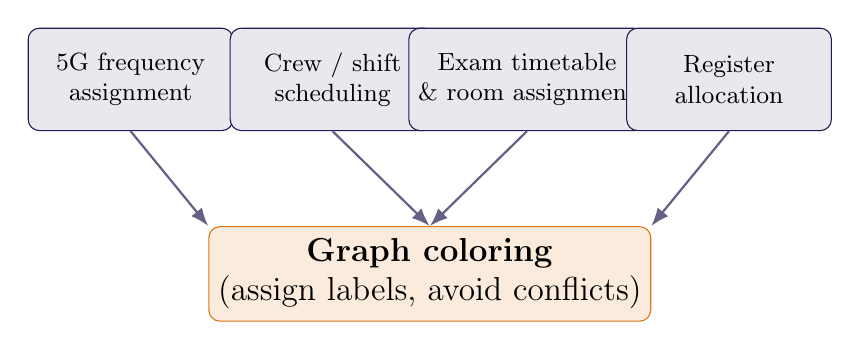
\begin{tikzpicture}[scale=0.95,
        ind/.style={rectangle,rounded corners,
                    draw=QCIcol1,fill=QCIcol1!10,
                    minimum width=2.6cm,minimum height=1.3cm,
                    align=center,font=\small}]
    \node[ind] (a) at (-4, 1.4) {5G frequency\\assignment};
    \node[ind] (b) at (-1.3, 1.4) {Crew / shift\\scheduling};
    \node[ind] (c) at ( 1.3, 1.4) {Exam timetable\\\& room assignment};
    \node[ind] (d) at ( 4.0, 1.4) {Register\\allocation};

    \node[rectangle,rounded corners,
          draw=qciorange,fill=qciorange!15,
          minimum width=5cm,minimum height=1.2cm,
          align=center,font=\large] (core) at (0, -1.2)
      {\textbf{Graph coloring}\\
       (assign labels, avoid conflicts)};

    \draw[-Latex,thick,QCIcol1!70] (a.south) -- (core.north west);
    \draw[-Latex,thick,QCIcol1!70] (b.south) -- (core.north);
    \draw[-Latex,thick,QCIcol1!70] (c.south) -- (core.north);
    \draw[-Latex,thick,QCIcol1!70] (d.south) -- (core.north east);
  \end{tikzpicture}

  \medskip
  \footnotesize
  Every problem above reduces to \alert{minimum vertex coloring}: assign
  one of $k$ labels per item so conflicting items differ. We want $k$ as
  small as possible.
\end{frame}

\begin{frame}{Why this matters at scale}
  \begin{block}{The economic stake}
    A 5G operator with 5000 antennas across a metro area must minimise
    spectrum use. \alert{Each saved frequency} translates to
    capacity that can be sold to subscribers.
  \end{block}

  \medskip
  Today's tooling:
  \begin{itemize}
    \item Greedy heuristics: fast, off by 20--40\% on dense networks.
    \item Exact solvers (CPLEX, Gurobi): exact, but \alert{don't scale}
          past a few dozen nodes on dense graphs.
    \item Custom column generation: scales but slow on the inner
          ``best next column'' subproblem.
  \end{itemize}

  \medskip
  \textbf{QCi's approach}: accelerate the inner subproblem on Dirac-3.
\end{frame}

% ===========================================================================
\section{Our approach}

\begin{frame}{The QCi pipeline}
  \centering
  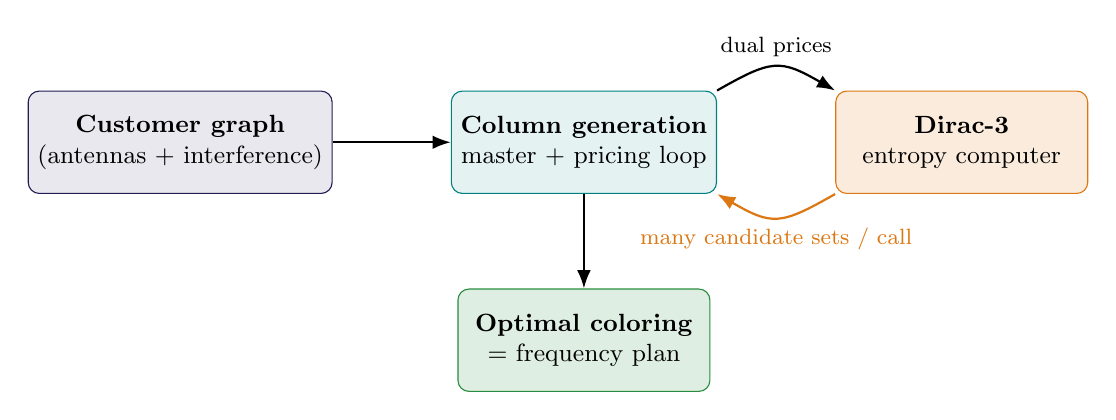
\begin{tikzpicture}[node distance=0.4cm,
                      box/.style={rectangle,rounded corners,
                                  minimum width=3.2cm,minimum height=1.3cm,
                                  align=center,font=\small}]
    \node[box,draw=QCIcol1,fill=QCIcol1!10] (g) {\textbf{Customer graph}\\
      (antennas + interference)};
    \node[box,draw=qciteal,fill=qciteal!10,right=1.5cm of g] (cg) {\textbf{Column generation}\\
      master + pricing loop};
    \node[box,draw=qciorange,fill=qciorange!15,right=1.5cm of cg] (dirac) {\textbf{Dirac-3}\\
      entropy computer};
    \node[box,draw=qcigreen,fill=qcigreen!15,below=1.2cm of cg] (out) {\textbf{Optimal coloring}\\
      = frequency plan};

    \draw[-Latex,thick] (g) -- (cg);
    \draw[-Latex,thick] (cg.north east) .. controls +(0.7,0.4) and +(-0.7,0.4) ..
      node[above,font=\footnotesize] {dual prices} (dirac.north west);
    \draw[-Latex,thick,qciorange] (dirac.south west) .. controls +(-0.7,-0.4) and +(0.7,-0.4) ..
      node[below,font=\footnotesize] {many candidate sets / call} (cg.south east);
    \draw[-Latex,thick] (cg) -- (out);
  \end{tikzpicture}

  \medskip
  \begin{itemize}\small
    \item No quantum compilation by the customer; the device is wrapped behind a
          Python API.
    \item One device call returns dozens of candidate assignments
          in parallel --- \alert{the wedge that beats classical CG}.
  \end{itemize}
\end{frame}

\begin{frame}{Dirac-3 in one slide}
  \begin{columns}[T]
    \begin{column}{0.55\textwidth}
      Dirac-3 is QCi's \textbf{entropy computer}: a photonic device that
      \emph{natively} optimises a continuous quadratic program in a
      single shot.

      \medskip
      \begin{itemize}\small
        \item Each call returns up to 100 high-quality solution candidates.
        \item No quantum-circuit compilation, no qubit-count bottleneck.
        \item Cloud-API access today; on-prem deployment available.
      \end{itemize}

      \medskip
      The hard combinatorial subproblem inside column generation maps
      \alert{directly} onto Dirac's native interface.
    \end{column}
    \begin{column}{0.45\textwidth}
      \centering
      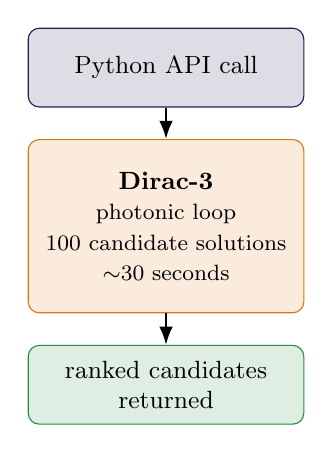
\begin{tikzpicture}[scale=0.9]
        \node[rectangle,rounded corners,
              draw=QCIcol1,fill=QCIcol1!15,
              minimum width=3.5cm,minimum height=1cm,align=center,
              font=\small] (api) {Python API call};
        \node[rectangle,rounded corners,
              draw=qciorange,fill=qciorange!15,
              minimum width=3.5cm,minimum height=2.2cm,align=center,
              font=\small,below=0.4cm of api]
              (dev) {\textbf{Dirac-3}\\
              \footnotesize photonic loop\\\footnotesize 100 candidate solutions\\
              \footnotesize $\sim$30 seconds};
        \node[rectangle,rounded corners,
              draw=qcigreen,fill=qcigreen!15,
              minimum width=3.5cm,minimum height=1cm,align=center,
              font=\small,below=0.4cm of dev]
              (out) {ranked candidates\\returned};
        \draw[-Latex,thick] (api) -- (dev);
        \draw[-Latex,thick] (dev) -- (out);
      \end{tikzpicture}
    \end{column}
  \end{columns}
\end{frame}

% ===========================================================================
\section{Results}

\begin{frame}{Head-to-head: same optimum, fewer iterations}
  \centering
  \renewcommand{\arraystretch}{1.25}
  \begin{tabular}{l c c c}
    \toprule
    \textbf{Method} & \textbf{Frequencies used} & \textbf{Wall time} & \textbf{Iterations}\\
    \midrule
    Greedy (DSATUR)        & 8       & $<\,$0.01\,s & ---\\
    Direct optimisation    & \alert{6}      & 0.04\,s & ---\\
    Classical CG           & \alert{6}       & 0.02\,s & 7\\
    \rowcolor{QCIcol3}
    \textbf{QCi Quantum CG} & \alert{6}      & 50\,s   & \textbf{4}\\
    \bottomrule
  \end{tabular}

  \medskip
  \footnotesize
  Synthetic 12-antenna interference network. All methods that reach $6$
  match the proven optimum. \alert{QCi Quantum CG converges in roughly
  half the iterations} of classical CG --- the gap widens on larger,
  denser instances where each iteration costs more.
\end{frame}

\begin{frame}{Where the wedge widens}
  \begin{block}{Benchmark suite (ER random graphs)}
    \begin{itemize}\small
      \item $n = 100, p = 0.5$: Quantum CG returns 2--4$\times$ more
            candidate solutions per call; converges in
            \alert{half the iterations}.
      \item $n = 100, p = 0.7$: classical solvers degrade quickly; QCG
            reaches the same chromatic number with a richer column pool.
      \item $n > 100$: classical exact methods time out;
            CG remains the only tractable path, and QCG accelerates the
            inner loop.
    \end{itemize}
  \end{block}

  \medskip
  \footnotesize
  Per-call latency on Dirac-3 cloud is currently
  $\sim$30--90\,s. Wall-clock advantage materialises when the classical
  alternative also takes minutes per iteration.
\end{frame}

% ===========================================================================
\section{Next steps}

\begin{frame}{What we deliver}
  \begin{itemize}
    \item A \alert{Python toolkit} that drops into existing planning
          workflows; the customer writes a NetworkX graph, the toolkit
          returns a coloring.
    \item \alert{Three backends} interchangeable behind one API:
      \begin{itemize}\small
        \item Cloud Dirac-3 (production today)
        \item On-prem Dirac-3 (pilot)
        \item Classical CG fallback (always available)
      \end{itemize}
    \item \alert{Reproducibility built-in}: recorded device calls can be
          replayed offline, so colleagues review the same results without
          burning device time.
  \end{itemize}
\end{frame}

\begin{frame}{Try it}
  \begin{block}{This bundle}
    \begin{itemize}
      \item 6 Jupyter notebooks (theory $\to$ end-to-end pipeline).
      \item 3 slide decks (this one, an end-to-end tutorial, a technical
            deep dive).
      \item All examples run \alert{offline} on bundled data; live device
            mode is one toggle away.
    \end{itemize}
  \end{block}

  \medskip
  \begin{center}
    \large\color{QCIcol1}
    \textbf{Contact:} \texttt{solutions@quantumcomputinginc.com}\\
    \medskip
    \footnotesize\color{QCIcol2}
    Quantum Computing Inc \quad|\quad quantumcomputinginc.com \quad|\quad (703) 436-2161
  \end{center}
\end{frame}

\end{document}
